\documentclass[aspectratio=169,11pt]{beamer}
% =====================================================================
% Who Pays When Firms Keep Losing?  -- revised 10-minute proposal deck
% Main deck: title + 9 slides (~10 min).  Overflow lives in the appendix
% behind hyperlink buttons.  Speaker notes (\note{}) carry the timing.
% =====================================================================

% ---------- Packages ----------
\usepackage[T1]{fontenc}
\usepackage{lmodern}
\usepackage{amsmath}
\usepackage{amssymb}          % \blacksquare (beamer loads it too; explicit is safer)
\usepackage{booktabs}
\usepackage{array}
\usepackage{tabularx}
\usepackage{appendixnumberbeamer}
\usepackage[most]{tcolorbox}
\usepackage{tikz}
\usetikzlibrary{positioning,arrows.meta,calc}

% ---------- Colors ----------
\definecolor{SlateTeal}{HTML}{1B4D5C}
\definecolor{WarmAmber}{HTML}{D4A84B}
\definecolor{DeepCharcoal}{HTML}{2C3E50}
\definecolor{SoftCoral}{HTML}{C0534D}
\definecolor{CoolGray}{HTML}{8899A6}
\definecolor{PaleSage}{HTML}{EDF2F0}

% ---------- Safe zone ----------
\newlength{\safezone}
\setlength{\safezone}{1.5cm}

% ---------- Theme ----------
\setbeamersize{text margin left=1.2cm, text margin right=1.2cm}
\setbeamertemplate{navigation symbols}{}
\setbeamercolor{normal text}{fg=DeepCharcoal,bg=white}
\setbeamercolor{frametitle}{fg=SlateTeal}
\setbeamercolor{structure}{fg=SlateTeal}
\setbeamercolor{alerted text}{fg=SoftCoral}
\setbeamercolor{footline}{fg=CoolGray}
\setbeamercolor{button}{bg=PaleSage,fg=SlateTeal}
\setbeamerfont{frametitle}{size=\Large,series=\bfseries}
\setbeamerfont{footline}{size=\scriptsize}
\setbeamertemplate{itemize item}{\color{WarmAmber}\raisebox{0.15ex}{\scriptsize$\blacksquare$}}
\setbeamertemplate{itemize subitem}{\color{CoolGray}\textendash}
\setbeamertemplate{enumerate item}{\color{SlateTeal}\bfseries\insertenumlabel.}

\setbeamertemplate{frametitle}{%
  \vskip18pt%
  \nointerlineskip%
  {\usebeamerfont{frametitle}\usebeamercolor[fg]{frametitle}\insertframetitle\par}%
  \vskip2pt%
  {\color{WarmAmber}\rule{\textwidth}{1.2pt}}%
  \vskip4pt%
}

\setbeamertemplate{footline}{%
  \begin{beamercolorbox}[wd=\paperwidth, ht=18pt, right, rightskip=\safezone]{footline}%
    \usebeamerfont{footline}\insertframenumber\,/\,\inserttotalframenumber\vskip6pt%
  \end{beamercolorbox}%
}

% appendixnumberbeamer's \translate in the bookmark string -> hyperref warning
\pdfstringdefDisableCommands{\def\translate#1{#1}}

% ---------- Boxes ----------
\newtcolorbox{keybox}[1][]{enhanced, colback=PaleSage, colframe=SlateTeal,
  boxrule=0pt, leftrule=3pt, arc=2pt, left=8pt, right=8pt, top=6pt, bottom=6pt,
  fontupper=\color{DeepCharcoal}, #1}
% main-deck cards use \small; appendix cards may pass fontupper=\footnotesize
\newtcolorbox{cardbox}[2][]{enhanced, colback=white, colframe=SlateTeal!35,
  boxrule=0.6pt, arc=2pt, left=6pt, right=6pt, top=4pt, bottom=5pt,
  title={#2}, coltitle=white, colbacktitle=SlateTeal, fonttitle=\bfseries\small,
  fontupper=\small\raggedright, before upper={\setlength{\itemsep}{1pt}},
  #1}
\newtcolorbox{accentbox}[1][]{enhanced, colback=WarmAmber!12, colframe=WarmAmber,
  boxrule=0.8pt, arc=2pt, left=8pt, right=8pt, top=5pt, bottom=5pt, #1}

\newcommand{\hl}[1]{{\color{WarmAmber}\bfseries #1}}
\newcommand{\muted}[1]{{\color{CoolGray}#1}}
\newcommand{\hy}[1]{\textbf{\textcolor{SlateTeal}{#1}}}

% ---------- TikZ styles (all defined here, none inside frames) ----------
\tikzset{
  % life-cycle diagram
  stage/.style={draw=SlateTeal, fill=PaleSage, rounded corners=2pt, line width=0.7pt,
    text width=2.55cm, minimum width=2.8cm, minimum height=1.2cm, align=center,
    font=\small\bfseries, text=SlateTeal,
    execute at begin node={\hyphenpenalty=10000\exhyphenpenalty=10000}},
  zombie/.style={stage, draw=SoftCoral, fill=SoftCoral!10, text=SoftCoral},
  exitnode/.style={stage, draw=WarmAmber, fill=WarmAmber!18, text=DeepCharcoal},
  note/.style={text width=2.75cm, minimum width=2.8cm, minimum height=1.1cm,
    align=center, anchor=north, font=\footnotesize, text=CoolGray,
    execute at begin node={\hyphenpenalty=10000\exhyphenpenalty=10000}},
  flow/.style={-{Stealth[length=2.2mm]}, line width=0.8pt, color=SlateTeal!70},
  % conjecture plot
  axis/.style={-{Stealth[length=1.8mm]}, line width=0.6pt, color=DeepCharcoal},
  tick/.style={line width=0.5pt, color=DeepCharcoal},
  ticklab/.style={font=\scriptsize, text=DeepCharcoal, minimum width=0.3cm,
    minimum height=0.3cm, inner sep=1pt},
  axlab/.style={font=\scriptsize, text=DeepCharcoal, minimum width=3.0cm,
    minimum height=0.35cm, inner sep=1pt},
  wcurve/.style={line width=1.6pt, color=SoftCoral},
  wthin/.style={line width=1.4pt, color=SoftCoral, dash pattern=on 4pt off 2pt},
  ocurve/.style={line width=1.6pt, color=SlateTeal},
  curvelab/.style={font=\scriptsize\bfseries, align=left, anchor=west,
    text width=1.6cm, minimum width=1.6cm, minimum height=0.35cm, inner sep=1pt},
  caveat/.style={font=\scriptsize\itshape, text=SoftCoral, minimum width=4.5cm,
    minimum height=0.35cm, inner sep=1pt},
}

% ---------- Title info ----------
\title{Who Pays When Firms Keep Losing?}
\subtitle{Workers, Owners, and Debt over the Distress Life Cycle}
\author{Research Proposal}
\date{}

\setbeamertemplate{title page}{%
  \vfill
  \begin{center}
    {\usebeamerfont{title}\Huge\bfseries\color{SlateTeal}\inserttitle\par}
    \vskip8pt
    {\color{WarmAmber}\rule{0.55\textwidth}{1.2pt}}
    \vskip8pt
    {\Large\color{DeepCharcoal}\insertsubtitle\par}
    \vskip22pt
    {\large\color{CoolGray}\insertauthor\par}
    \vskip4pt
    {\small\color{CoolGray}Canadian linked worker--firm--owner data, 2001--2019\par}
  \end{center}
  \vfill
}

\begin{document}

% ======================================================
% 1. TITLE  (~0:15)
\begin{frame}[plain]
  \titlepage
  \note{~0:15. One sentence: ``I want to know who pays when a private firm keeps losing money, and when.''}
\end{frame}

% ======================================================
% 2. MOTIVATION  (~1:00)
\begin{frame}{Insurance against losses has to be paid for}
  \begin{columns}[T,onlytextwidth]
    \column{0.52\textwidth}
    \textbf{What we know}
    \begin{itemize}
      \item Workers capture a \hl{small share} of firm gains \muted{(Card et al.\ 2018; Kline et al.\ 2019)}
      \item But they bear a \alert{larger share} of losses, mainly via job loss \muted{(Wang \& Young 2025)}
      \item Firms \hl{partly insure} workers against firm shocks \muted{(Guiso, Pistaferri \& Schivardi 2005; Balke \& Lamadon 2022)}
    \end{itemize}

    \column{0.44\textwidth}
    \begin{keybox}
      \textbf{The gap.}\\[3pt]
      Insurance is not free. When a firm \emph{keeps} losing money, someone funds it:
      \begin{itemize}
        \item owners' equity
        \item new debt
        \item workers, once the firm can no longer pay
      \end{itemize}
      \vspace{2pt}
      \textbf{Who, and when?}
    \end{keybox}
  \end{columns}
  \note{~1:00. Left column is the known asymmetry: small share of gains, larger share of losses.
    Right column is the gap: insurance has to be financed by someone. End on ``who, and when?''}
\end{frame}

% ======================================================
% 3. QUESTION + STAKES  (~1:00)
\begin{frame}[label=question]{I ask who absorbs a firm's persistent losses, and when}
  \vspace{2pt}
  \begin{keybox}
    \large When a private firm's value added falls \hl{persistently}, how is the loss divided among
    \textbf{incumbent workers}, \textbf{future workers}, \textbf{owners}, and the firm's \textbf{debt}?
    How does this division change as the firm moves from a first loss into \alert{prolonged distress} and \textbf{exit}?
  \end{keybox}
  \vspace{6pt}
  \begin{accentbox}
    \textbf{Why it matters:} does protecting distressed firms protect their \emph{workers}, or only delay and shift the losses?
  \end{accentbox}
  \vfill
  {\small\muted{Sub-questions: timing $\cdot$ thin buffers $\cdot$ gain/loss asymmetry $\cdot$ zombie exit}}%
  \hfill\hyperlink{subq}{\beamerbutton{Sub-questions}}\,\hyperlink{whocares}{\beamerbutton{Who cares}}\hspace{\safezone}
  \note{~1:00. Read the question slowly once. Then the policy stakes: forbearance and bailouts keep
    firms alive, but do they protect workers or just move the losses later? Do not walk through the
    four sub-questions; they are in the appendix.}
\end{frame}

% ======================================================
% 4. THREE VIEWS -> TENSION  (~1:00)
\begin{frame}{Theory disagrees: owners, workers, or lenders pay}
  \begin{columns}[T,onlytextwidth]
    \column{0.315\textwidth}
    \begin{cardbox}[fontupper=\footnotesize\raggedright]{Owners absorb}
      \textbf{Insurance view}\\[2pt]
      Risk-neutral owners smooth wages; losses hit profits and equity.\\[3pt]
      \muted{Azariadis; Baily; Guiso et al.}
    \end{cardbox}

    \column{0.315\textwidth}
    \begin{cardbox}[fontupper=\footnotesize\raggedright]{Workers bear}
      \textbf{Job-loss view}\\[2pt]
      Firms cut jobs rather than wages; displacement costs are large.\\[3pt]
      \muted{Wang \& Young; Bertheau et al.; Graham et al.}
    \end{cardbox}

    \column{0.315\textwidth}
    \begin{cardbox}[fontupper=\footnotesize\raggedright]{Lenders absorb}
      \textbf{Zombie view}\\[2pt]
      Credit keeps unviable firms alive and \emph{prevents} layoffs.\\[3pt]
      \muted{Caballero, Hoshi \& Kashyap; Acharya et al.}
    \end{cardbox}
  \end{columns}

  \vspace{6pt}
  \begin{keybox}
    \textbf{Conjecture:} all three hold, \hl{at different stages}.
    The answer is about \textbf{timing}, which has not been measured directly.
  \end{keybox}
  \note{~1:00. Each view names a different payer. They look contradictory, but each is a
    snapshot at a different stage. Measuring the timing reconciles them; that is what is new.}
\end{frame}

% ======================================================
% 5. LIFE CYCLE  (~0:45)
\begin{frame}{Losses travel through a distress life cycle to exit}
  \vspace{10pt}
  \centering
  % Coordinate map (positioning library; node distance 0.55cm; all nodes 2.8cm x 1.2cm):
  %   s1 First persistent loss  x = 0      (origin, centre)
  %   s2 Repeated losses        x = 3.35cm (2.8 + 0.55)
  %   s3 Zombie stage           x = 6.70cm
  %   s4 Exit                   x = 10.05cm   -> total width ~12.85cm < 13.6cm textwidth
  %   n1..n4 notes: 2.8cm wide, anchor=north, 0.2cm below each stage's south anchor
  %   arrows s1->s2->s3->s4 run along y = 0 between node borders (no labels)
  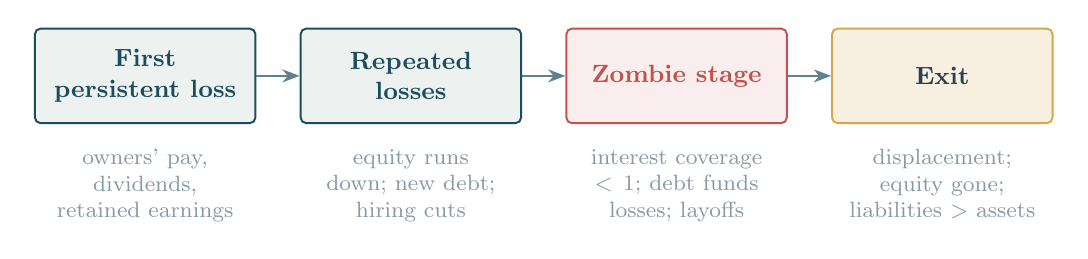
\begin{tikzpicture}[node distance=0.55cm]
    \node[stage]                       (s1) {First persistent loss};
    \node[stage, right=of s1]          (s2) {Repeated losses};
    \node[zombie, right=of s2]         (s3) {Zombie stage};
    \node[exitnode, right=of s3]       (s4) {Exit};
    \draw[flow] (s1) -- (s2);
    \draw[flow] (s2) -- (s3);
    \draw[flow] (s3) -- (s4);
    \node[note] at ($(s1.south)+(0,-0.2)$) (n1) {owners' pay, dividends, retained earnings};
    \node[note] at ($(s2.south)+(0,-0.2)$) (n2) {equity runs down; new debt; hiring cuts};
    \node[note] at ($(s3.south)+(0,-0.2)$) (n3) {interest coverage $<1$; debt funds losses; layoffs};
    \node[note] at ($(s4.south)+(0,-0.2)$) (n4) {displacement; equity gone; liabilities $>$ assets};
  \end{tikzpicture}

  \vspace{16pt}
  \raggedright
  {\muted{I follow the same firms, workers, and owners through all four stages.}}
  \note{~0:45. Walk left to right in one breath: owners' buffers first, then debt, then the
    zombie stage with coverage below one, then exit. Zombie is a stage, not a treatment.}
\end{frame}

% ======================================================
% 6. DATA  (~0:45)
\begin{frame}[label=data]{CEEDD links each firm to its workers, books, and owners}
  \vspace{6pt}
  \begin{columns}[T,onlytextwidth]
    \column{0.315\textwidth}
    \begin{cardbox}{Workers: T4 + ROE}
      \begin{itemize}
        \item earnings
        \item \hl{layoffs vs quits}
        \item hires
      \end{itemize}
    \end{cardbox}
    \column{0.315\textwidth}
    \begin{cardbox}{Firm: NALMF}
      \begin{itemize}
        \item value added
        \item \hl{balance sheets}
      \end{itemize}
    \end{cardbox}
    \column{0.315\textwidth}
    \begin{cardbox}{Owners: Schedule 50}
      \begin{itemize}
        \item \hl{chained ownership} to individuals
      \end{itemize}
    \end{cardbox}
  \end{columns}

  \vspace{10pt}
  \begin{keybox}
    Canadian private firms, 2001--2019: workers, owners, and debt of the \emph{same} firm.
  \end{keybox}
  \vfill
  \hfill\hyperlink{datamap}{\beamerbutton{Data map}}\hspace{\safezone}
  \note{~0:45. Get credit for the data: linked owners are what make a full incidence
    accounting possible. Variable-level detail is in the appendix data map.}
\end{frame}

% ======================================================
% 7. ACCOUNTING IN WORDS, THEN MATH  (~1:15)
\begin{frame}[label=accounting]{Every lost dollar must show up on someone's ledger}
  \textbf{Value added before interest is the ``pie''}: its size does not depend on how it is split.
  So a loss has to land somewhere, in two senses:

  \vspace{10pt}
  \begin{columns}[c,onlytextwidth]
    \column{0.36\textwidth}
    \hy{1.\ Who gets less income?}\\
    {\small\muted{workers, lenders, owners, government}}
    \column{0.62\textwidth}
    \[
      \Delta(\text{VA}+\text{Int}) = \underbrace{\Delta \text{Payroll}}_{\text{workers}}
      + \underbrace{\Delta \text{Int}}_{\text{lenders}}
      + \underbrace{\Delta \Pi + \Delta \text{CCA}}_{\text{owners, gov't}}
    \]
  \end{columns}

  \vspace{8pt}
  \begin{columns}[c,onlytextwidth]
    \column{0.36\textwidth}
    \hy{2.\ Who funds the shortfall?}\\
    {\small\muted{new debt or owners' equity}}
    \column{0.62\textwidth}
    \[
      \Delta \text{Assets} = \underbrace{\Delta \text{Liabilities}}_{\text{debt}} + \underbrace{\Delta \text{Equity}}_{\text{owners}}
    \]
  \end{columns}
  \note{~1:15. Say it in words first: if the pie shrinks, someone's slice shrinks (income),
    and the hole is financed by borrowing or by running down equity (funding).
    Only then point at the identities. Each braced term becomes an event-study outcome.}
\end{frame}

% ======================================================
% 8. ESTIMAND + PICTURE OF THE CONJECTURE  (~1:30)
\begin{frame}[label=conjecture]{Conjecture: owners and debt pay first, workers later}
  \begin{columns}[c,onlytextwidth]
    \column{0.41\textwidth}
    \begin{keybox}[fontupper=\color{DeepCharcoal}\small\raggedright]
      \textbf{Estimand:} share of the cumulative loss borne by claimant $g$ by horizon $h$
      \[
        \theta_g(h)=\frac{\sum_{k=0}^{h}\beta^{(g)}_k}{\sum_{k=0}^{h}\beta^{(\text{VA}+\text{Int})}_k}
      \]
      \footnotesize $\beta_k$: event-time-$k$ change vs.\ matched firms.\\[2pt]
      Estimated separately for losses and gains, and by the firm's \hl{buffer} at $t-2$.
    \end{keybox}

    \column{0.56\textwidth}
    \centering
    % Coordinate map (cm; origin = axes corner; 1 year = 0.9cm in x, share 1 = 3.6cm in y):
    %   x-axis: (0,0) -> (4.8,0); ticks h=0..5 at x = 0,0.9,...,4.5; tick labels at y=-0.25
    %   x-axis label: centre (2.25,-0.75)
    %   y-axis: (0,0) -> (0,3.95); y-axis label rotated 90, centre (-0.4,1.8)
    %   caveat line: centre (2.25,4.35)  (0.4cm above y-axis tip)
    %   curves on h in [0,5] (stylized functional forms, NOT data):
    %     Workers (thin buffer): 0.08+0.75(1-e^{-h/1.2}); h=0 -> y=0.29, h=5 -> y=2.95
    %     Workers:               0.08+0.60(1-e^{-h/2.5}); h=0 -> y=0.29, h=5 -> y=2.16
    %     Owners + debt:         0.90-0.65(1-e^{-h/2.5}); h=0 -> y=3.24, h=5 -> y=1.22
    %   end labels (anchor west, x=4.6): y=2.95 / 2.16 / 1.22  -> gaps 0.79 / 0.94cm
    %   label right edge = 4.6+1.6 = 6.2cm; picture width ~6.8cm < 7.75cm column
    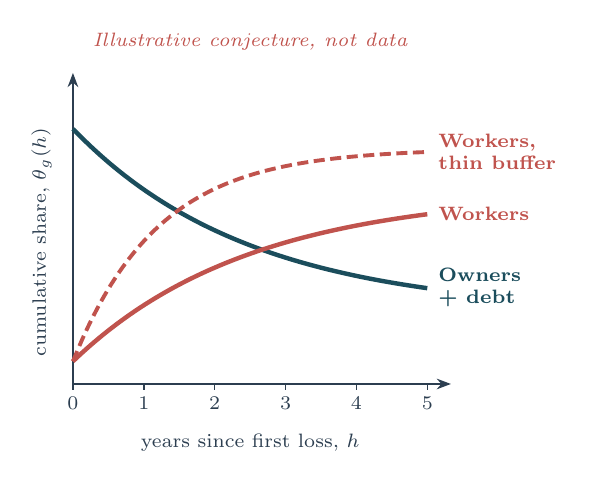
\begin{tikzpicture}
      \draw[axis] (0,0) -- (4.8,0);
      \draw[axis] (0,0) -- (0,3.95);
      \foreach \h in {0,1,2,3,4,5} {
        \draw[tick] ({0.9*\h},0) -- ({0.9*\h},-0.08);
        \node[ticklab] at ({0.9*\h},-0.25) {\h};
      }
      \node[axlab] at (2.25,-0.75) {years since first loss, $h$};
      \node[axlab, rotate=90] at (-0.4,1.8) {cumulative share, $\theta_g(h)$};
      \draw[ocurve] plot[domain=0:5, samples=40, smooth]
        ({0.9*\x},{3.6*(0.90-0.65*(1-exp(-\x/2.5)))});
      \draw[wcurve] plot[domain=0:5, samples=40, smooth]
        ({0.9*\x},{3.6*(0.08+0.60*(1-exp(-\x/2.5)))});
      \draw[wthin] plot[domain=0:5, samples=40, smooth]
        ({0.9*\x},{3.6*(0.08+0.75*(1-exp(-\x/1.2)))});
      \node[curvelab, text=SoftCoral] at (4.6,2.95) {Workers,\\thin buffer};
      \node[curvelab, text=SoftCoral] at (4.6,2.16) {Workers};
      \node[curvelab, text=SlateTeal] at (4.6,1.22) {Owners\\+ debt};
      \node[caveat] at (2.25,4.35) {Illustrative conjecture, not data};
    \end{tikzpicture}
  \end{columns}
  \vfill
  \hfill\hyperlink{hyp}{\beamerbutton{Hypotheses}}\hspace{\safezone}
  \note{~1:30. Define theta in words: of all the value added lost so far, what fraction shows
    up as lower payroll, lower owner income, or new debt. Then the picture: the conjecture is
    that the workers' line starts low and rises over 3--5 years, and rises sooner when the
    buffer is thin. Stress: these curves are drawn by hand, not estimated.}
\end{frame}

% ======================================================
% 9. DESIGN + VULNERABILITIES  (~1:15)
\begin{frame}[label=design]{The design measures incidence, not causal effects}
  \begin{columns}[T,onlytextwidth]
    \column{0.48\textwidth}
    \begin{cardbox}{What I estimate}
      \begin{itemize}
        \item Stacked event studies of persistent value-added falls (and rises)
        \item Matched control firms; intention-to-treat incumbents
        \item Exit: displacement design by distress duration
      \end{itemize}
    \end{cardbox}
    \column{0.48\textwidth}
    \begin{cardbox}[colbacktitle=SoftCoral, colframe=SoftCoral!45]{What the design can't do}
      \begin{itemize}
        \item Value-added falls are \alert{not random}: results are incidence \emph{accounting} vs matched firms, not causal effects of exogenous shocks
        \item No lender data: ``debt-funded'' and a creditor-shortfall \emph{bound}, not creditor losses
        \item Zombie status is a \emph{stage}, never a treatment
      \end{itemize}
    \end{cardbox}
  \end{columns}
  \note{~1:15. Be explicit. The comparison is firms with a persistent fall vs matched firms
    without one; incumbents are followed whether or not they stay (ITT). Then pause on the
    biggest vulnerability: the fall is not random, so this is accounting, not a causal effect.}
\end{frame}

% ======================================================
% 10. BOTTOM LINE + WHAT WOULD CHANGE MY MIND  (~1:15)
\begin{frame}[label=closing]{Bottom line: the answer is about timing}
  \begin{keybox}
    \large Measuring $\theta_g(h)$ from first loss to exit tells us whether protecting distressed
    firms protects their \textbf{workers}, or only \hl{delays and shifts} the losses.
  \end{keybox}
  \vspace{4pt}
  \begin{columns}[T,onlytextwidth]
    \column{0.48\textwidth}
    \begin{cardbox}{What would change my mind}
      If the workers' share does \alert{not} rise with the horizon, the timing story fails:
      lead with financing + exit instead.
    \end{cardbox}
    \column{0.48\textwidth}
    \begin{cardbox}{Feedback I would like}
      \begin{itemize}
        \item Is accounting vs matched firms convincing enough?
        \item Export shocks: appendix validation, or more?
      \end{itemize}
    \end{cardbox}
  \end{columns}
  \vfill
  \hfill\hyperlink{nextsteps}{\beamerbutton{First three months}}\,\hyperlink{contrib}{\beamerbutton{Contribution}}\hspace{\safezone}
  \note{~1:15. Land the one sentence in the box. Then say what result would be most
    informative: a flat workers' share would kill the timing story, and the paper would lead
    with financing and exit. Close by asking for the two pieces of feedback.}
\end{frame}

% ======================================================
\appendix
\begin{frame}[plain]
  \vfill
  \begin{center}
    {\Huge\bfseries\color{SlateTeal}Appendix\par}
    \vskip8pt
    {\color{WarmAmber}\rule{0.3\textwidth}{1.2pt}}
  \end{center}
  \vfill
\end{frame}

% ======================================================
\begin{frame}[label=subq]{Four sub-questions organize the analysis}
  \begin{enumerate}
    \item \textbf{Timing:} Do losses reach workers immediately, or only after owners' buffers run out?
    \item \textbf{State dependence:} Does a thin financial buffer move losses onto workers sooner?
    \item \textbf{Asymmetry:} Do gains rebuild owners' equity while losses end up with workers?
    \item \textbf{Exit:} When a long-distressed (``zombie'') firm finally dies, who pays?
  \end{enumerate}
  \vfill
  \hfill\hyperlink{question}{\beamerbutton{Back}}\hspace{\safezone}
\end{frame}

% ======================================================
\begin{frame}[label=whocares]{The answer matters to labor, finance, and policy}
  \begin{columns}[T,onlytextwidth]
    \column{0.315\textwidth}
    \begin{cardbox}{Labor economists}
      \begin{itemize}
        \item \emph{Why} is downside incidence asymmetric?
        \item Where does firm insurance stop?
      \end{itemize}
    \end{cardbox}

    \column{0.315\textwidth}
    \begin{cardbox}{Finance \& zombies}
      \begin{itemize}
        \item Zombie work measures aggregate costs, not workers' incomes
        \item Links debt to worker outcomes
      \end{itemize}
    \end{cardbox}

    \column{0.315\textwidth}
    \begin{cardbox}{Policy}
      \begin{itemize}
        \item Forbearance, bailouts, bankruptcy timing
        \item Survival \hl{moves losses} across time
      \end{itemize}
    \end{cardbox}
  \end{columns}
  \vfill
  \hfill\hyperlink{question}{\beamerbutton{Back}}\hspace{\safezone}
\end{frame}

% ======================================================
\begin{frame}[label=hyp]{Five testable predictions follow from the conjecture}
  \small
  \renewcommand{\arraystretch}{1.2}
  \begin{tabularx}{\textwidth}{p{0.8cm} >{\raggedright\arraybackslash}X >{\raggedright\arraybackslash}p{3.6cm}}
    \toprule
     & \textbf{Prediction} & \textbf{Evidence} \\
    \midrule
    \hy{H1} & Deferred incidence: workers' share of a persistent loss is small at impact and rises over 3--5 years & $\theta_{\text{workers}}(h)$ increasing in $h$ \\
    \hy{H2} & Thin buffers (low equity, prior losses, coverage $<1$) pass losses to workers sooner & Interactions with buffer at $t-2$ (descriptive) \\
    \hy{H3} & Gains rebuild retained earnings; losses end with workers; asymmetry grows with $h$ & $\theta_g(h)$ for rises vs falls \\
    \hy{H4} & Longer distress before exit: more pre-exit erosion, smaller owner loss, bigger creditor gap & Exit design by distress duration \\
    \hy{H5} & Hiring falls before incumbents' earnings & Timing of hires vs incumbents \\
    \bottomrule
  \end{tabularx}
  \vfill
  \hfill \hyperlink{conjecture}{\beamerbutton{Back}}\hspace{\safezone}
\end{frame}

% ======================================================
\begin{frame}[label=contrib]{This proposal adds financing and dynamics to exit}
  \footnotesize
  \renewcommand{\arraystretch}{1.15}
  \begin{tabularx}{\textwidth}{>{\raggedright\arraybackslash}p{3.0cm} >{\raggedright\arraybackslash}X >{\raggedright\arraybackslash}X}
    \toprule
    \textbf{Closest paper} & \textbf{What it does} & \textbf{\color{SlateTeal}What this paper adds} \\
    \midrule
    Wang \& Young (2025) & Worker vs owner incidence; asymmetry via job loss (U.S.\ S-corps) & \hl{Financing} of losses; \hl{dynamics} to exit; new hires; layoffs vs quits \\
    Azzalini (2026) & Negative pass-through rises in \emph{recessions} & State = the \emph{firm's own} buffer, on its balance sheet \\
    Malgieri \& Citino (2025) & Constrained firms pass through more & Buffer \emph{evolves} with losses; followed to exit \\
    Graham et al.\ (2023) & Worker losses \emph{at} bankruptcy & The \emph{years before} exit; owners and creditors alongside \\
    Acharya et al.\ (NY Fed) & Zombie credit prevents layoffs (aggregate) & Incomes of zombie firms' \emph{own} workers and owners \\
    \bottomrule
  \end{tabularx}
  \vfill
  \hfill \hyperlink{closing}{\beamerbutton{Back}}\hspace{\safezone}
\end{frame}

% ======================================================
\begin{frame}[label=nextsteps]{Next: check identities, clean exits, test timing}
  \begin{enumerate}
    \item Check that the accounting identities hold firm by firm
    \item Clean false exits (restructurings, new business numbers)
    \item Does the workers' share \hl{rise with the horizon}? If not, lead with financing + exit
  \end{enumerate}
  \vspace{8pt}
  \muted{Optional: export shocks as an appendix validation.}
  \vfill
  \hfill \hyperlink{closing}{\beamerbutton{Back}}\hspace{\safezone}
\end{frame}

% ======================================================
\begin{frame}[label=datamap]{Every claimant maps to observed CEEDD variables}
  \small
  \renewcommand{\arraystretch}{1.2}
  \begin{tabularx}{\textwidth}{>{\raggedright\arraybackslash}p{3.2cm} >{\raggedright\arraybackslash}X}
    \toprule
    \textbf{Claimant / margin} & \textbf{CEEDD variables} \\
    \midrule
    Incumbent workers & T4 earnings; ROE separation reason (shortage of work vs quit); EI \\
    Future workers & First T4 year at firm; ROE start month (if separated); hires' AKM effects \\
    Owners & Schedule 50 chained shares; owner and family T4 pay; dividends declared; $\Delta$ retained earnings \\
    Debt & Total, current, long-term liabilities; interest and bank charges \\
    Distress stage & Interest coverage; loss carryforward; equity; incorporation date \\
    Exit & Last PD7 remittance month (cleaned of successor firms) \\
    \bottomrule
  \end{tabularx}
  \vfill
  \hfill \hyperlink{data}{\beamerbutton{Back}}\hspace{\safezone}
\end{frame}

\end{document}
